\documentclass[UTF8]{ctexart}

%固定图片位置
\usepackage{float}

%插入超链接
\usepackage{url}

\usepackage{tikz,mathpazo}
\usetikzlibrary{shapes.geometric, arrows}
\usetikzlibrary{calc}


\usepackage{listings}
%插入代码的配置
\definecolor{CPPLight}  {HTML} {686868}
\definecolor{CPPSteel}  {HTML} {888888}
\definecolor{CPPDark}   {HTML} {262626}
\definecolor{CPPBlue}   {HTML} {4172A3}
\definecolor{CPPGreen}  {HTML} {487818}
\definecolor{CPPBrown}  {HTML} {A07040}
\definecolor{CPPRed}    {HTML} {AD4D3A}
\definecolor{CPPViolet} {HTML} {7040A0}
\definecolor{CPPGray}  {HTML} {B8B8B8}
\lstset{
	language=Python,                                     % 设置语言
    columns=fixed,    
    breaklines = true,   
    basicstyle=\small ,
    numbers=left,                                        % 在左侧显示行号
    %frame=none,                                          % 不显示背景边框
    backgroundcolor=\color[RGB]{245,245,244},            % 设定背景颜色
    keywordstyle=\color[RGB]{40,40,255},                 % 设定关键字颜色
    numberstyle=\tiny\color{darkgray},           % 设定行号格式
    %commentstyle=\it\color[RGB]{0,96,96},                % 设置代码注释的格式
    stringstyle=\rmfamily\slshape\color[RGB]{128,0,0},   % 设置字符串格式
    showstringspaces=false,                              % 不显示字符串中的空格                           
    %morekeywords={True,alignas,continute,friend,register,true,alignof,decltype,goto,
    %reinterpret_cast,try,asm,defult,if,return,typedef,auto,delete,inline,short,
    %typeid,bool,do,int,signed,typename,break,double,long,sizeof,union,case,
    %dynamic_cast,mutable,static,unsigned,catch,else,namespace,static_assert,using,
    %char,enum,new,static_cast,virtual,char16_t,char32_t,explict,noexcept,struct,
    %void,export,nullptr,switch,volatile,class,extern,operator,template,wchar_t,
    %const,false,private,this,while,constexpr,float,protected,thread_local,
    %const_cast,for,public,throw,std,rand},
    emph={access,and,break,class,continue,def,del,elif ,else,%
	except,exec,finally,for,from,global,if,import,in,i s,%
	lambda,not,or,pass,print,raise,return,try,while},
    emphstyle=\color{CPPViolet}, 
    emph={[2]True, False, None, self},
	emphstyle=[2]\color{green},
	emph={[3]from, import, as},
	emphstyle=[3]\color{blue},
	upquote=true,
	morecomment=[s]{"""}{"""},
	commentstyle=\color{orange}\slshape,
	emph={[4]1, 2, 3, 4, 5, 6, 7, 8, 9, 0},
	emphstyle=[4]\color{red},
	emph={[5]numpy, np, plt},
	emphstyle=[5]\color{red},
	literate=*{:}{{\textcolor{blue}:}}{1}%
	{=}{{\textcolor{blue}=}}{1}%
	{-}{{\textcolor{blue}-}}{1}%
	{+}{{\textcolor{blue}+}}{1}%
	{*}{{\textcolor{blue}*}}{1}%
	{!}{{\textcolor{blue}!}}{1}%
	{(}{{\textcolor{blue}(}}{1}%
	{)}{{\textcolor{blue})}}{1}%
	{[}{{\textcolor{blue}[}}{1}%
	{]}{{\textcolor{blue}]}}{1}%
	{<}{{\textcolor{blue}<}}{1}%
	{>}{{\textcolor{blue}>}}{1},%
	framexleftmargin=0.1mm, framextopmargin=0.1mm, frame=shadowbox, rulesepcolor=\color{black},
}



\usepackage{geometry}
\geometry{left=2cm, right=2cm, top=1.2cm, bottom=1.2cm}

%得到引用的标题内容
\usepackage{nameref} 

%添加首行缩进,两个字符
\usepackage{indentfirst}
\setlength{\parindent}{2em}

%多行公式一个编号
\usepackage{amsmath}

%文献引用,标准类型为plain
%\usepackage[hyperref=true,backend=biber,sorting=none,backref=true]{biblatex}
%\addbibresource{ref.bib}
\bibliographystyle{plain}
\usepackage{cite}

\pagestyle{plain}

%跨页表格
\usepackage{multirow}
\usepackage{longtable,booktabs}
\usepackage{supertabular}
\usepackage{makecell}

%调整itemize等的间距
\usepackage{enumitem}


\usepackage{graphicx}

%超链接
\usepackage[linkcolor=yellow,citecolor=red,backref=page,hyperfootnotes=true]{hyperref}
\hypersetup{
bookmarks=true,
colorlinks=true,
linkcolor=black
}
\usepackage{tabularx} %This package must be placed after package {hyperref}, otherwise footnote marks are NOT treated as hyperlinks.


%引入了一些改进的数学环境,如align
\usepackage{amsmath}

\title{数据结构:表达式树}
\author{姓名:鲁国锐 \protect\newline
\and 学号:17020021031 \\
\and 专业:电子信息科学与技术}


\begin{document}
	\maketitle
	\renewcommand{\contentsname}{Contents}
	\tableofcontents
	\newpage
	
	\hypersetup{
	bookmarks=true,
	colorlinks=true,
	linkcolor=red,
	urlcolor=blue
	}
	\section{问题分析}
	\subsection{题目描述}
	\indent 表达式树的树叶是操作数($operand$),而其他的节点为操作符($operator$)。比如下面 的示例:
	
	代表:中缀表达式:$(a+b)*(c*(d+e))$以及相应的后缀表达式:$ab+cde+**$。
	
	作业要求输入一个中缀表达式,构建其相应的表达式树,并输出验证。
	\begin{itemize}
		\item 样例输入:(a+b)*(c*(d+e)
		
		\item 样例输出:(格式可修改为更加美观的图形化输出)

				$\times$
			
			$+$                   $\times$
			
			$a$      $b$      $c$      $+$
			
			$d$     $e$
	
	\end{itemize}
	
	
	请测试至少三组不同输入。
	
	提示:先将中缀表达式转换为后缀表达式,然后结合栈(stack)构造表达式树。
	
	

	\subsection{问题分析}
	\indent 根据题目,我们需要解决的问题有:
	\begin{enumerate}[leftmargin=50pt]
	\item 设计输入输出流程并对输入表达式的合法性进行检查(见\ref{input and output}节);
	\item 实现函数$to\_RPN$将中缀表达式转换为后缀表达式(见\ref{fun to RPN}节);
	\item 用后缀表达式构建表达式树(见\ref{con tree}节)。
	\end{enumerate}
	

	
	\section{解决方案}
		\subsection{设计输入输出流程}\label{input and output}
		\indent 因为考虑到操作数可能是多位数,所以方便起见我们用$string$来表示操作数和运算符,并将它们存在一个$vector$中。而为了能够将每一个$string$分开,我们规定所有的操作数和运算符之间必须用空格分隔。
		
		\indent 对于输出,根据表达式树的特性:\textbf{对其进行后序遍历并输出得到的是一个后缀表达式},我们可以先将得到的后缀表达式输出一遍,再对构造好的表达式树后序遍历输出一次,稍微调整一下缩进,使输出的两个表达式对齐,可以很方便地检查二者是否一致。
		
		\indent 为了使程序能够正常运行并退出,我们还要对输入进行检查以确保它的合法性,防止在程序执行过程中出现数组越界等情况。不过时间有限,这里我主要考虑了以下几种情况:
		\begin{enumerate}
			\item 输入中有非法字符;
			\item 两字符之间没有加空格;
			\item 括号未匹配。
		\end{enumerate}
	
		\indent 由于我们再判断两个运算符的优先级时用到了数组,所以以上三种情况可能会导致数组的下标越界。至于解决方案因为涉及到将中缀表达式转换为后缀表达式的方法,我们放在下一节中介绍。
	
		\subsection{将中缀表达式转换为后缀表达式}\label{fun to RPN}
		
		\indent 关于怎么将中缀表达式转换为后缀表达式的算法,课本\cite{data_structure}上有比较详细的介绍,但在这里我们仍需要对其进行修改和补充以适应我们自己的要求。
		
		\indent 在开始实现$to\_RPN$函数前我们首先要实现一个比较运算符之间优先级的函数$order$。这里我们借鉴课本\cite{data_structure}上的做法,用一个枚举类型的变量将各个运算符的英文表示换成数字。然后用一个二维数组来表示两个运算符之间的优先级关系。为了方便把原始的运算符跟其英文表示对应起来,这里我们还用了一个$map$把它们一一对应起来。这样我们在比较两个运算符时,只需要把它们作为$key$值传入$map$得到其英文表示对应的数字,再将数字作为下标传给数组来搜寻二者的优先级关系即可。
				
		\indent 到这里我们就可以阐述一下\ref{input and output}节中提到的第一种和第二种情况的解决方法了。如果输入中有非法字符,那么我们在$map$中是找不到对应的$key$值的,所以我们在对原始运算符进行转换之前要先在$map$中查找一遍,若没有这个$key$值,需要抛出一个异常,终止函数的进行并让用户重新输入。而对于第二种情况,操作数和运算符因为中间缺少空格而连在了一起,我们在对这个了“连体儿”进行判断时,认为它是操作符,显然作为运算符它是不合法的,这样就把第二种情况化归成了第一种情况。
		
		\indent 接下来就是中缀表达式转后缀表达式的具体算法了。这里我们需要借用一个运算符栈$optr$。首先我们从前往后遍历存放中缀表达式的$vector$,若:
		\begin{enumerate}
			\item 当前扫到的是操作数,直接将它接到要返回的结果$RPN$后面;
			\item 当前扫到的是运算符,则开始判断$optr$栈顶运算符和当前运算符之间的优先级关系,若:
			\begin{enumerate}
				\item 栈顶运算符优先级低于当前运算符,将当前运算符压入栈中,令下标$i$增一,开始访问下一元素;
				\item 栈顶运算符优先级与当前运算符一样,弹出栈顶元素,令下标$i$增一,开始访问下一元素;
				\item 栈顶运算符优先级高于当前运算符,弹出栈顶元素并把它接入$RPN$,此时不能令下标自增,而是要继续比较当前运算符与栈中下一运算符的优先级关系。
				\item 不是以上任何一种情况,说明两个本不可能相邻的运算符碰到了一起,这就是\ref{input and output}节中所说的第三种情况:括号未匹配。注意这里右括号以及空字符的优先级是最低的,而左括号的优先级是最高的,所以其它任何栈顶运算符遇到了右括号或空字符都会被弹出,任何当前运算符遇到左括号都会被压入。如果括号正常匹配的话,左括号或右括号是不会遇到空字符的,而一旦遇到,则说明括号一定没有匹配上。因此我们在数组中给这些情况赋一个其它的值,以便检查括号的匹配情况。
			\end{enumerate}

		\end{enumerate}	
		
		\indent 注意这里我们以空字符表示表达式的开始与结束,所以我们在一开始先将一个空字符入栈,同时给输入的最后接上一个空字符。这样我们重复以上操作直至最后两个空字符相遇,栈内的所有元素被弹出,同时输入也已遍历到了最后,整个转换过程就此结束,返回的$RPN$即为后缀表达式。
		
		\subsection{构建表达式树}\label{con tree}
		\indent 仔细分析一下我们可以发现,\textbf{构建表达式树的过程其实和后缀表达式求值的过程是一样的}。表达式树中的每一个含运算符的节点都可视作是它的两个孩子用它进行运算后的结果。所以我们直接按照后缀表达式求值的过程来构建表达式树即可。
		
		\indent 我们从前往后遍历得到的后缀表达式,如果当前元素是操作数,用其构建一个节点压入辅助栈中;如果当前元素是运算符,则弹出一个或两个元素(视该运算符是单目还是双目而定),分别作为右孩子和左孩子接在以当前元素构建的节点上,再将新构建的节点压回栈中。注意先弹出的接为右孩子,后弹出的接为左孩子。如此反复直至遍历完整个后缀表达式,此时栈中应当还剩下一个元素,即为表达式树的根节点。我们对其进行后序遍历并输出,得到的结果应与后缀表达式一致。
		
		
	
	\section{算法设计}
	见图\ref{to RPN}、图\ref{main}\footnote{为使流程图相对简洁,未在其中画出捕获异常的过程。}。


\begin{figure}[H]
	\centering 
	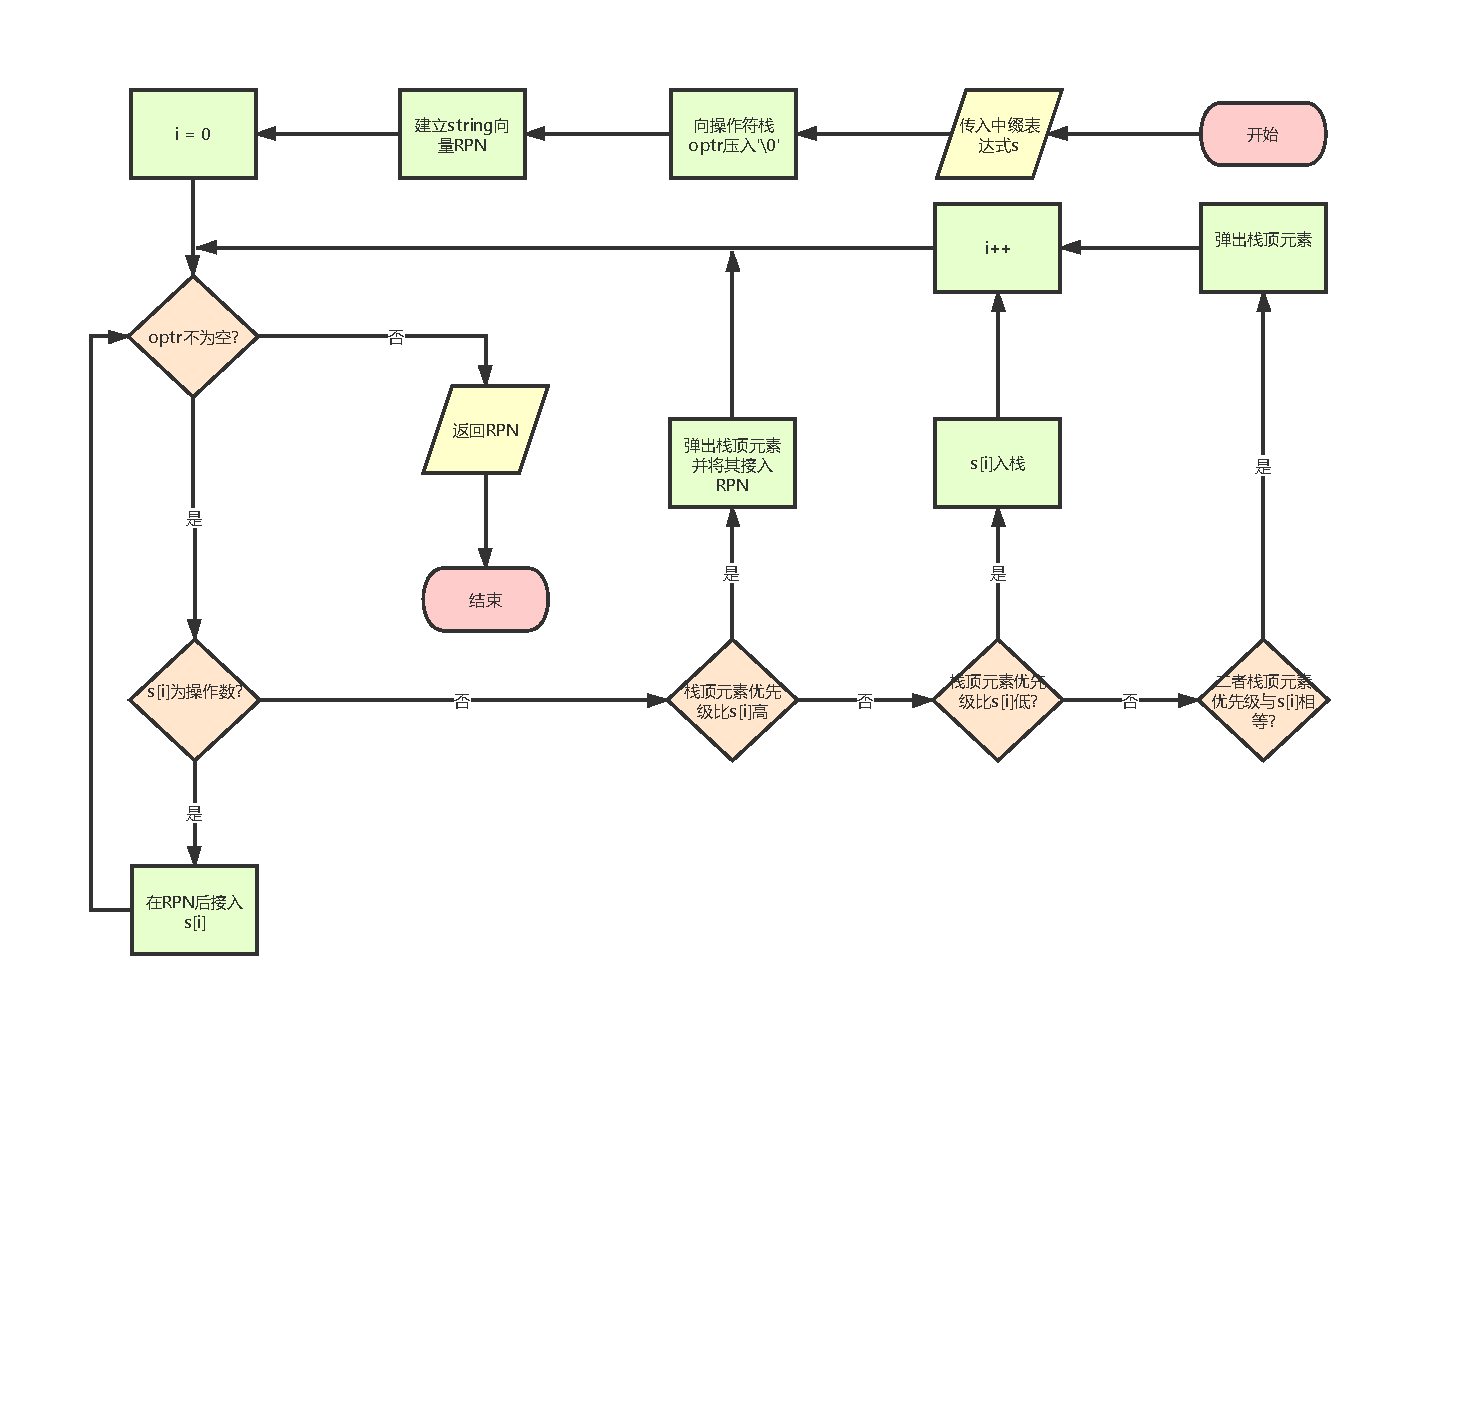
\includegraphics[width=20cm, height=19cm]{to_RPN.pdf} 
	\caption{$to\_RPN$函数流程图} 
	\label{to RPN}
\end{figure}



\begin{figure}[H]
	\centering 
	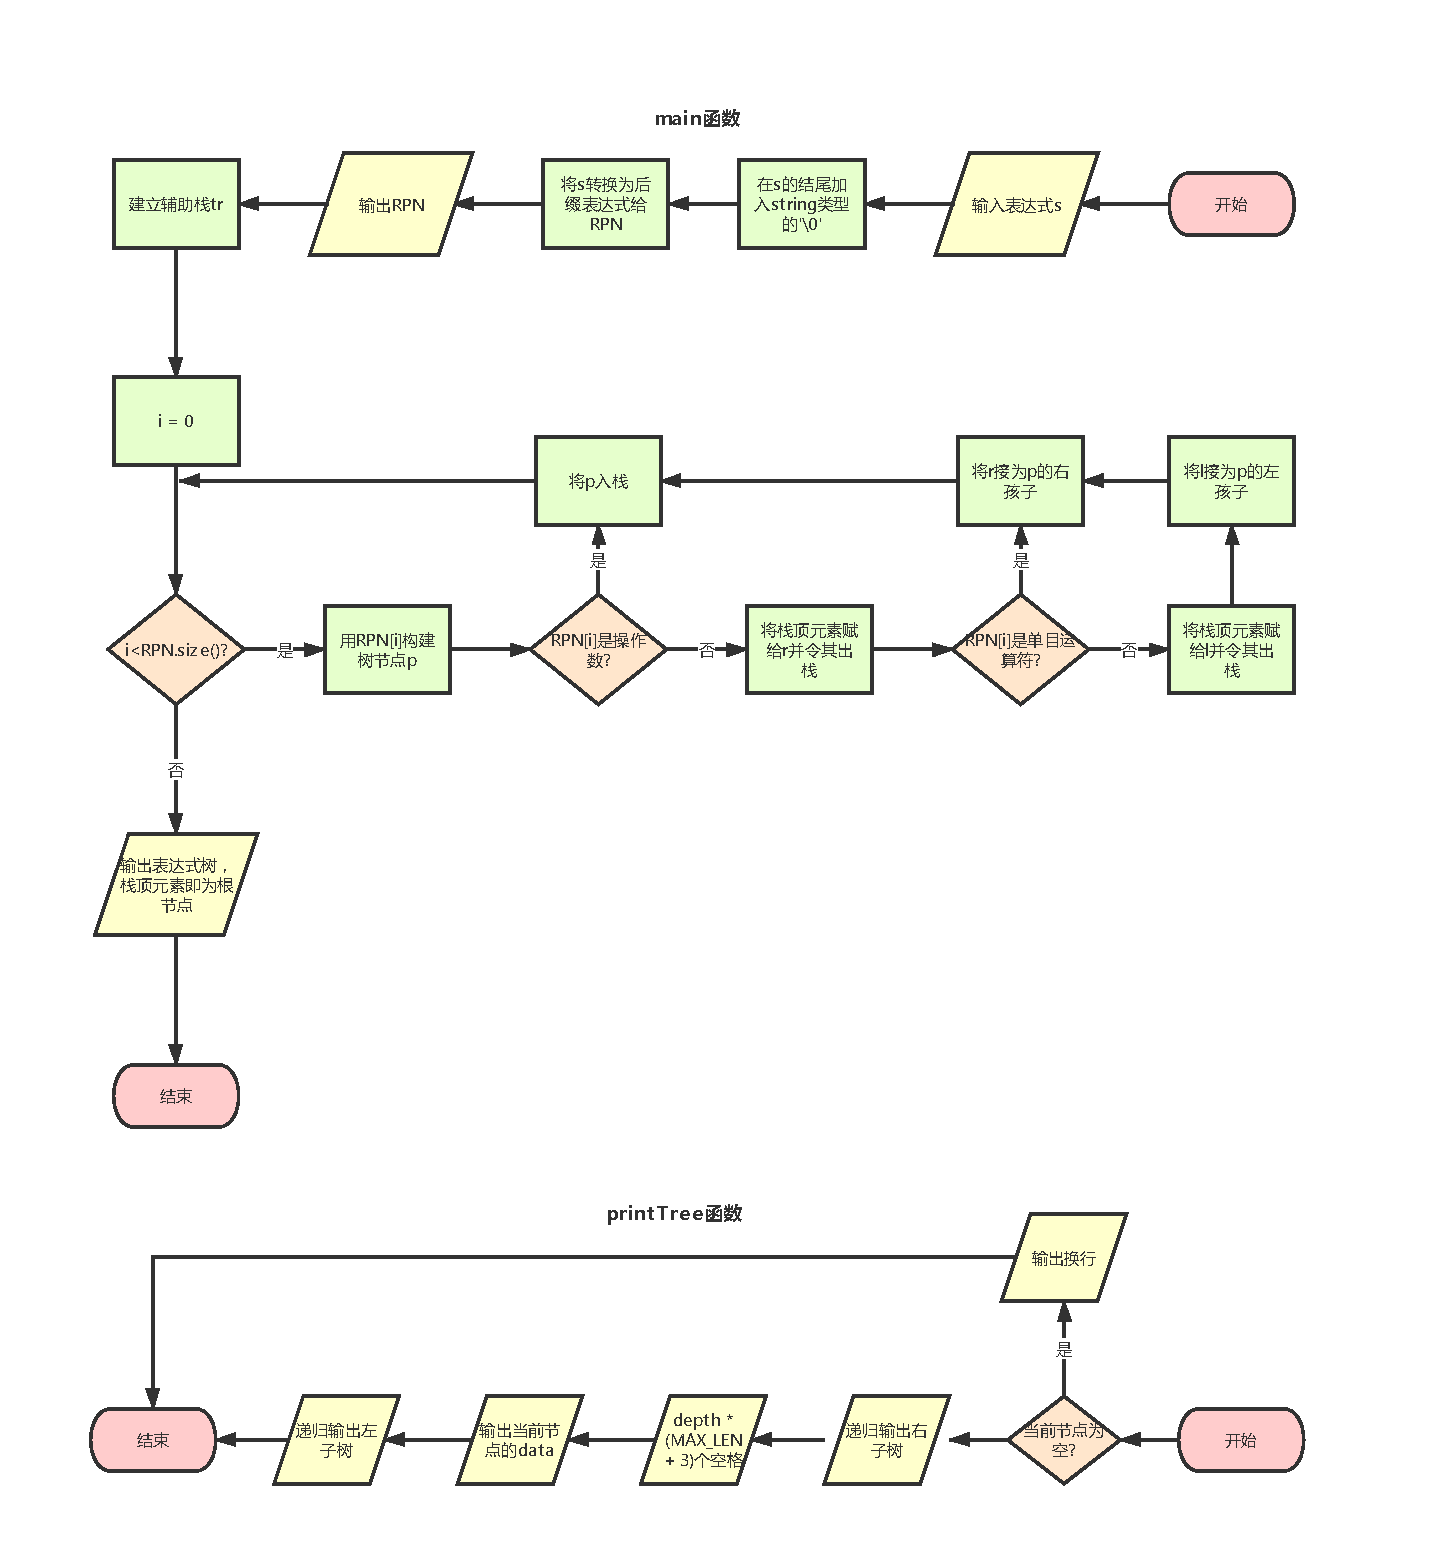
\includegraphics[width=20cm, height=23cm]{expression_tree_main.pdf} 
	\caption{$main$函数流程图} 
	\label{main}
\end{figure}
\newpage



	\section{编程实现\protect \footnotemark[1]}
	\footnotetext[1]{代码也可从该网址得到:\url{https://github.com/chenfeng123456/CourseInOUC/blob/master/algorithm/expression_tree/expression_tree.cpp}}

	\begin{lstlisting}[language=C++,caption={expression\_tree代码},label={expression_tree_code}]
#include <iostream>
#include <string>
#include <stack>
#include <vector>
#include <typeinfo>
#include <map>
#include <stdio.h>


using namespace std;
#define N_OPTR 9
typedef enum { ADD, SUB, MUL, DIV, POW, FAC, L_P, R_P, EOE } Operator;
//             +    -    *    /    ^    !    (    )    \0

const char pri[N_OPTR][N_OPTR] =
{
'>',   '>',   '<',   '<',   '<',   '<',   '<',   '>',   '>',
'>',   '>',   '<',   '<',   '<',   '<',   '<',   '>',   '>',
'>',   '>',   '>',   '>',   '<',   '<',   '<',   '>',   '>',
'>',   '>',   '>',   '>',   '<',   '<',   '<',   '>',   '>',
'>',   '>',   '>',   '>',   '>',   '<',   '<',   '>',   '>',
'>',   '>',   '>',   '>',   '>',   '>',   ' ',   '>',   '>',
'<',   '<',   '<',   '<',   '<',   '<',   '<',   '=',   ' ',
' ',   ' ',   ' ',   ' ',   ' ',   ' ',   ' ',   ' ',   ' ',
'<',   '<',   '<',   '<',   '<',   '<',   '<',   ' ',   '='
};


#define IsRoot ( !((x).parent))
#define IsLc(x) ( ! IsRoot(x) && ( &(x) == (x).parent->lc))
#define IsRc(x) ( ! IsRoot(x) && ( &(x) == (x).parent->rc))
//#define FromParentTo(x) (IsRoot(x)

char order(string a, string b)
{
static map<string, int> symbols;
symbols["+"] = ADD;
symbols["-"] = SUB;
symbols["*"] = MUL;
symbols["/"] = DIV;
symbols["^"] = POW;
symbols["!"] = FAC;
symbols["("] = L_P;
symbols[")"] = R_P;
symbols["\\0"] = EOE;

char res = '\0';
if (symbols.find(a) != symbols.end() && symbols.find(b) != symbols.end())
res = pri[symbols[a]][symbols[b]];
else
throw "Illegal expresssion!";

return res;
}

template <typename T>
class Node
{
public:
T data;
Node<T> *parent;
Node<T> *lc;
Node<T> *rc;
int height;

Node() : parent(NULL), lc(NULL), rc(NULL), height(0) {}
Node(T e, Node<T> *p=NULL, Node<T> *l=NULL, Node<T> *r=NULL, int h=0) :
data(e), parent(p), lc(l), rc(r), height(h) {}
Node<T> *insertAsLc(Node<T> *e);
Node<T> *insertAsRc(Node<T> *e);
//~Node(){if(!parent) {remove(this);cout << "All nodes have been removed" << endl;}}
};
template <typename T>
Node<T>* Node<T>::insertAsLc(Node<T> *e)
{
lc = e;
e->parent = this;
return e;
}
template <typename T>
Node<T>* Node<T>::insertAsRc(Node<T> *e)
{
rc = e;
e->parent = this;
return e;
}



template <typename T>
void travPost(Node<T> *x)
{
if (!x) return;
travPost(x->lc);
travPost(x->rc);
cout << x->data << " ";
}

bool isdigit(string s)
{
int i = 0;
while ((s[i] >= '0' && s[i] <= '9') || (s[i] >= 'a' && s[i] <= 'z') || (s[i] >= 'A' && s[i] <= 'Z') || s[i] == '.')
{
i++;
}
return (i == s.length());
}

vector<string> toRPN(vector<string> s)
{
vector<string> RPN;
stack<string> optr;
optr.push("\\0");
int i = 0;
while (!optr.empty())
{
if (isdigit(s[i]))
{
RPN.push_back(s[i]);
i++;
}
else
{
char r;
try
{
r = order(optr.top(), s[i]);
}catch(const char* msg)
{
throw "Illegal expression!";
return RPN;
}
switch (r)
{
case '<':
{
optr.push(s[i]);
i++;
break;
}
case '=':
{
optr.pop();
i++;
break;
}
case '>':
{
string op = optr.top();
optr.pop();
RPN.push_back(op);
break;
}
default :
{
throw "Illegal expression!";
}
}
}
}

return RPN;
}


template <typename T>
void rm(Node<T> *x)
{
if (!x) return;
rm(x->lc);
rm(x->rc);
delete x;
}

template <typename T>
void remove(Node<T> *x)
{
if (x->parent)
{
if (x == x->parent->lc)
x->parent->lc = NULL;
if (x == x->parent->rc)
x->parent->rc = NULL;
}
rm(x);
}


int main()
{
cout << "姓名:鲁国锐" << endl;
cout << "学号:17020021031" << endl;
cout << endl;

vector<string> s;
vector<string> RPN;
while(1)
{
string c;
while(cin >> c)
{
s.push_back(c);
}
s.push_back("\\0");

try
{
RPN = toRPN(s);
}catch(const char* msg)
{
cerr << msg <<endl;
cin.clear();
cin.sync();
s.clear();
continue;
}
break;
}


cout << "后缀表达式:            ";
for (int i=0; i < RPN.size(); i++)
cout << RPN[i] << " ";
cout << endl;

stack<Node<string>*> tr;
for (int i=0; i < RPN.size(); i++)
{
string temp_op = RPN[i];
Node<string> *p = new Node<string>(temp_op);
if (isdigit(temp_op))
tr.push(p);
else
{
Node<string> *r = tr.top();
tr.pop();
// For unary operator such as "!".
// If they are placed at the second place
// then we shouldn't perform the operation
// of top() or pop() on the tr. Otherwise,
// it will be runtime error.
Node<string> *l;
if (!tr.empty())
l = tr.top();
if (temp_op != "!")
{
tr.pop();
}
p->insertAsRc(r);
if (temp_op != "!") p->insertAsLc(l);
tr.push(p);
}
}

cout << "对表达式树进行后序遍历:";
travPost(tr.top());
cout << endl;
remove(tr.top());

return 0;
}



	\end{lstlisting}

	\section{结果分析}
	\subsection{结果展示}

\begin{figure}[H]
	\centering 
	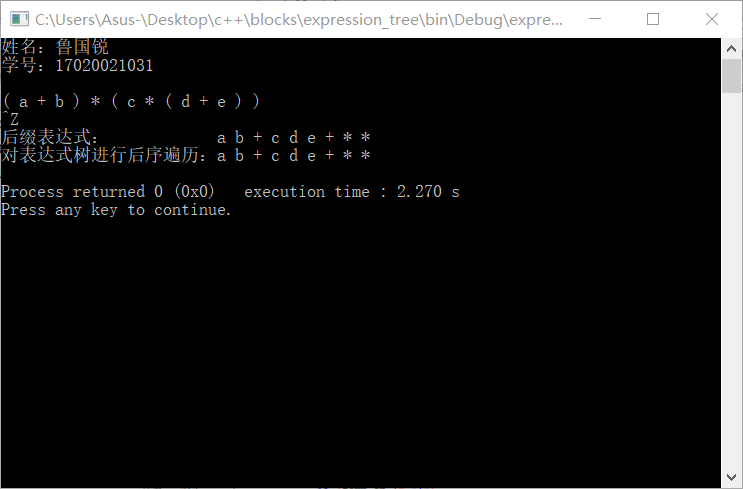
\includegraphics[scale=0.85]{res1.png} 
	\caption{结果1} 
	\label{res1}
\end{figure}

\begin{figure}[H]
	\centering 
	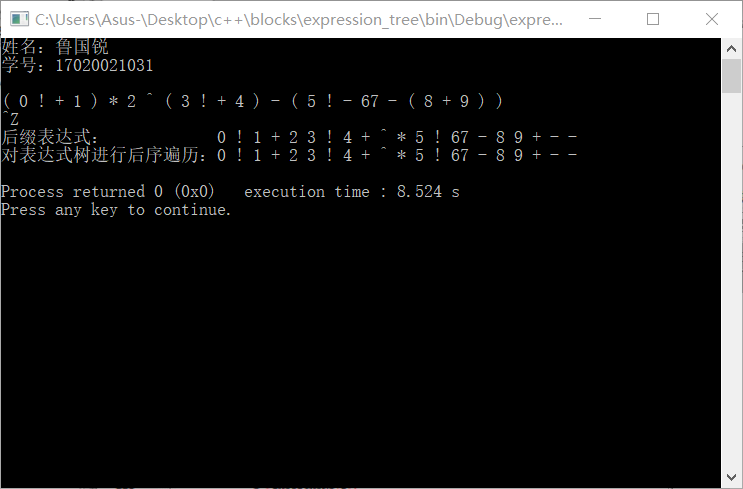
\includegraphics[scale=0.85]{res2.png} 
	\caption{结果2} 
	\label{res2}
\end{figure}

\begin{figure}[H]
	\centering 
	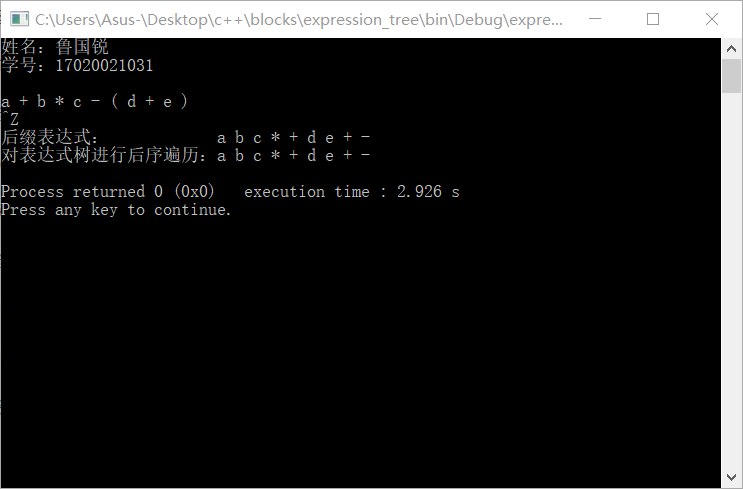
\includegraphics[scale=0.85]{res3.png} 
	\caption{结果3} 
	\label{res3}
\end{figure}

\begin{figure}[H]
	\centering 
	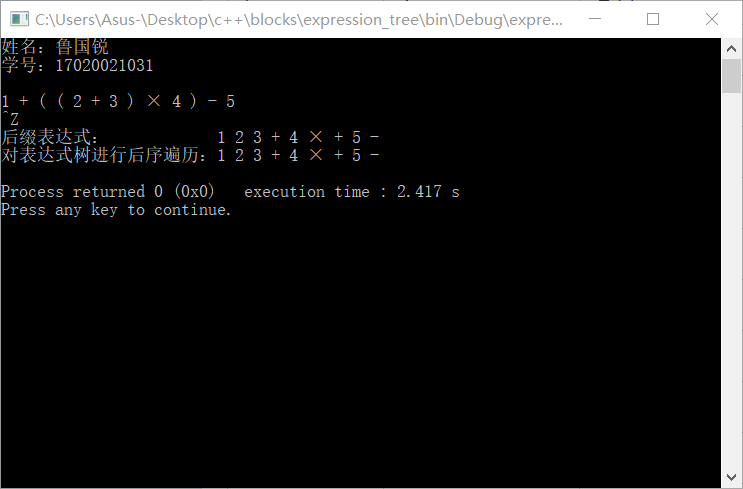
\includegraphics[scale=0.85]{res4.png} 
	\caption{结果4} 
	\label{res4}
\end{figure}

\begin{figure}[H]
	\centering 
	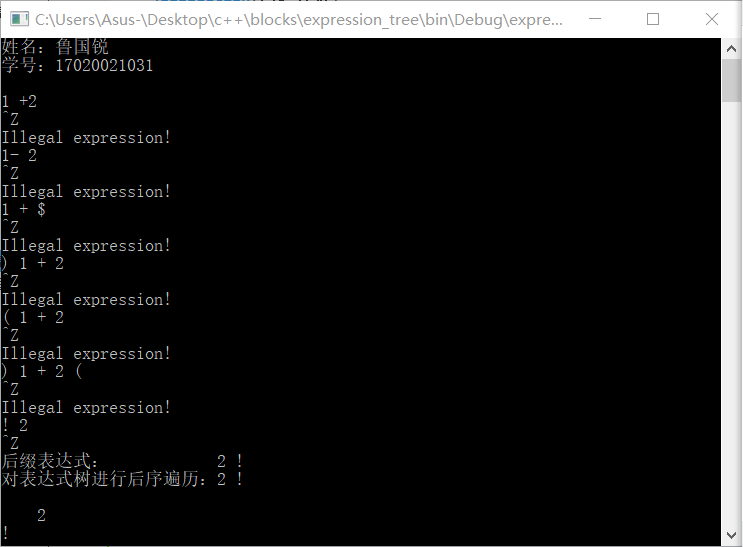
\includegraphics[scale=0.85]{res5.png} 
	\caption{结果5} 
	\label{res5}
\end{figure}

	\subsection{分析}\label{time_of_PrintLots}
	\indent 从最后一张图中可以看出,仍有部分非法输入的情况代码无法分辨出来,但因为它们并不会导致诸如数组越界这样的错误,程序可以正常运行、退出,再加之时间有限,故没有再去单独考虑这些情况。
	

	\section{总结体会}
	\indent 在完成此次作业的过程中遇到了很多问题,其中有两个比较隐蔽的$bug$,不太容易发现,在此稍作总结。
	\subsection{被忽略的空字符}
	\indent 在实现$to\_RPN$的过程中,我发现数组总会越界,找了很久的原因,最后发现是栈内和输入末端的空字符没有起作用。分析其原因大概是由于$string$本质上是一个字符数组,而我将一个空字符作为一个字符串,系统在扫到空字符的时候就停止了,所以导致最后比较优先级时会出现意外的结果。
	
	\subsection{循环析构}
	\indent 对于树或者链表的析构,应当放在树类或链表类中进行。因为如果把析构函数放在节点类中的话,程序最后要释放每一个节点,调用其析构函数,而在析构函数中又会对节点自身进行$delete$操作,从而再次触发对析构函数的调用,形成死循环。所以$delete$操作必须放在节点外进行。

\bibliography{ref.bib}
\end{document}